Untis er et fleksibelt skemalægningsprogram, som både er nemt at bruge, og giver mange muligheder for brugeren. Untis giver bl.a. mulighed for at brugeren kan bestemme, hvordan skemaet skal se ud uge for uge. Brugeren kan vælge om ugerne skal være A- og B-uger, altså eksempelvis, hvis der gennemsnitligt skal være 5 matematiklektioner på en uge, kan brugeren via A- og B-uger-funktionen gør således at der kommer 4 matematiklektioner i en uge, og 6 i en anden. Desuden har brugeren mulighed for at ændre skemaet, hvis nødvendigt i udvalgte uger, og bibeholde de resterende uger som faste og ensartede. 
Untis giver brugeren flere muligheder for at lægge skema, heriblandt manuel skemalægning, automatisk skemalægning samt optimering og en blanding af de nævnte. Dette sker ved at brugeren udfylder udvalgte brikker, og herefter benytter Untis til at udfylde resten for at opnå det bedste mulige resultat. Efter de manuelle indtastninger er udført, tager programmet stilling til de angivne parametre og forsøger at levere det bedste skema. Hvis der opstår konflikter, vil Untis informere brugeren og og vise hvori problemet ligger, så brugeren har nemt ved at rette fejlene og justere parametrene. Desuden tager programmet hensyn til indtastede data før programmet begynder at generere mulige skemaer, for at sikre at brugeren har indtastet korrekte eller realistiske antal af eksempelvis lokaler, lærer, klasser mm.\footfullcite{untis2016}
\begin{figure}[!h]
  \centering
  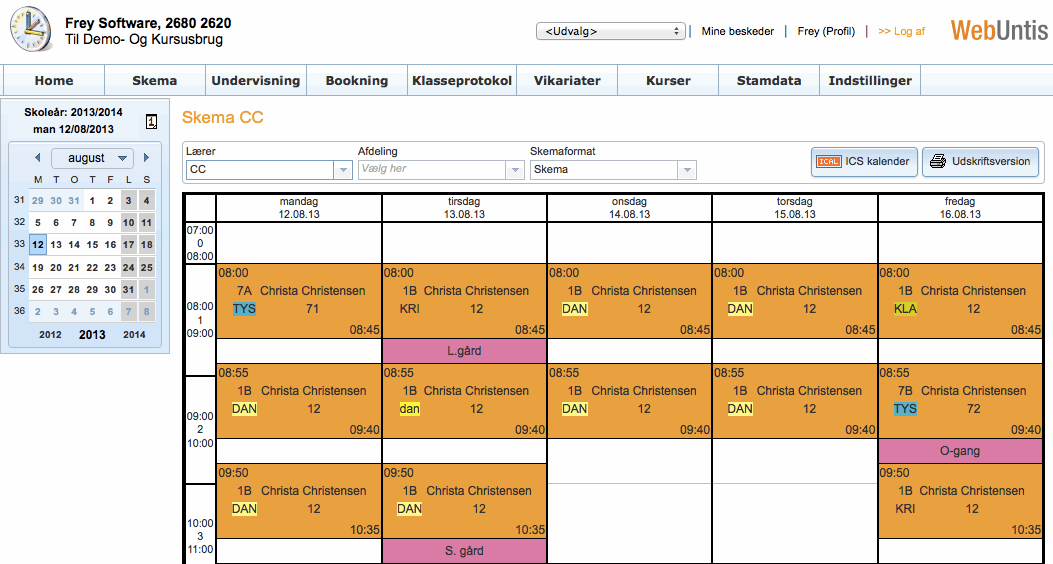
\includegraphics[width=\textwidth]{partials/graphics/untis.png}
  \caption{Eksempel på skemplanlægning i Untis.\footfullcite{untisb}}
  \label{fig:untis}
\end{figure}
